
\documentclass{beamer}
\usecolortheme{dove}
\setbeamertemplate{navigation symbols}{}
\usepackage{amsmath,amssymb,amsfonts,amsthm, multicol, subfigure, color}
\usepackage{bm}
\usepackage{graphicx}
\usepackage{tabularx}
\usepackage{booktabs}
\usepackage{hyperref}
\usepackage{pdfpages}
\usepackage{xcolor}
\definecolor{seagreen}{RGB}{46, 139, 87}
\def\independenT#1#2{\mathrel{\rlap{$#1#2$}\mkern2mu{#1#2}}}
\newcommand\indep{\protect\mathpalette{\protect\independenT}{\perp}}
\def\log{\text{log}}
\newcommand\logit{\text{logit}}
\newcommand\iid{\stackrel{\text{iid}}{\sim}}
\newcommand\E{\text{E}}
\newcommand\V{\text{V}}
\renewcommand\P{\text{P}}
\newcommand{\Cov}{\text{Cov}}
\newcommand{\Cor}{\text{Cor}}
\newcommand\doop{\texttt{do}}
\usepackage{stackrel}
\usepackage{tikz}
\usetikzlibrary{arrows,shapes.arrows,positioning,shapes,patterns,calc}
\newcommand\slideref[1]{\vskip .1cm \tiny \textcolor{gray}{{#1}}}
\newcommand\red[1]{\color{red}#1}
\newcommand\blue[1]{\color{blue}#1}
\newcommand\gray[1]{\color{gray}#1}
\newcommand\seagreen[1]{\color{seagreen}#1}
\newcommand\purple[1]{\color{purple}#1}
\newcommand\orange[1]{\color{orange}#1}
\newcommand\black[1]{\color{black}#1}
\newcommand\white[1]{\color{white}#1}
\newcommand\teal[1]{\color{teal}#1}
\newcommand\magenta[1]{\color{magenta}#1}
\newcommand\Fuchsia[1]{\color{Fuchsia}#1}
\newcommand\BlueGreen[1]{\color{BlueGreen}#1}
\newcommand\bblue[1]{\textcolor{blue}{\textbf{#1}}}
\newcommand\bred[1]{\textcolor{red}{\textbf{#1}}}
\newcommand\bgray[1]{\textcolor{gray}{\textbf{#1}}}
\newcommand\bgreen[1]{\textcolor{seagreen}{\textbf{#1}}}
\newcommand\bref[2]{\href{#1}{\color{blue}{#2}}}
\colorlet{lightgray}{gray!40}
\pgfdeclarelayer{bg}    % declare background layer for tikz
\pgfsetlayers{bg,main} % order layers for tikz
\newcommand\mycite[1]{\begin{scriptsize}\textcolor{darkgray}{(#1)}\end{scriptsize}}
\newcommand{\tcframe}{\frame{
%\small{
\only<1|handout:0>{\tableofcontents}
\only<2|handout:1>{\tableofcontents[currentsubsection]}}
%}
}

\usepackage[round]{natbib}
\bibliographystyle{humannat-mod}
\setbeamertemplate{enumerate items}[default]
\usepackage{mathtools}
\usepackage{ulem}

% Need to add examples

\newcommand{\goalsframe}{\begin{frame}{Learning goals for today}
At the end of class, you will be able to:
\begin{enumerate}
\item Study effects of policies in a spooky setting:\\when there is no matching control unit
\end{enumerate} \vskip .2in
\end{frame}}

\title{Difference in difference}
\author{INFO/STSCI/ILRST 3900: Causal Inference}
\date{31 Oct 2023}

\begin{document}

\maketitle

\goalsframe

\begin{frame}
Card, D., \& Krueger, A. B. (1994).\\\bref{https://davidcard.berkeley.edu/papers/njmin-aer.pdf}{Minimum Wages and Employment: A Case Study of the Fast-Food Industry in New Jersey and Pennsylvania.}\\The American Economic Review, 84(4), 772-793.
\end{frame}

\begin{frame}{Economic theory}
When the minimum wage rises, how might employment change? \pause
\begin{itemize}
\item employees cost more \pause
\item employers might get by with fewer employees
\end{itemize}
\end{frame}

\begin{frame}{The setting} \pause
\begin{itemize}
\item Federal minimum wage
\begin{itemize}
\item \$3.80 on April 1, 1990
\item \$4.25 on April 1, 1991
\end{itemize} \pause
\item New Jersey minimum wage
\begin{itemize}
\item \$5.05 on April 1, 1992
\end{itemize}
\end{itemize}
\end{frame}

\begin{frame}{NJ introduces a high minimum wage.\\How would you study the effect on employment?}{Source: \href{https://commons.wikimedia.org/wiki/File:New_Jersey_in_United_States_(zoom).svg}{Wikimedia}}
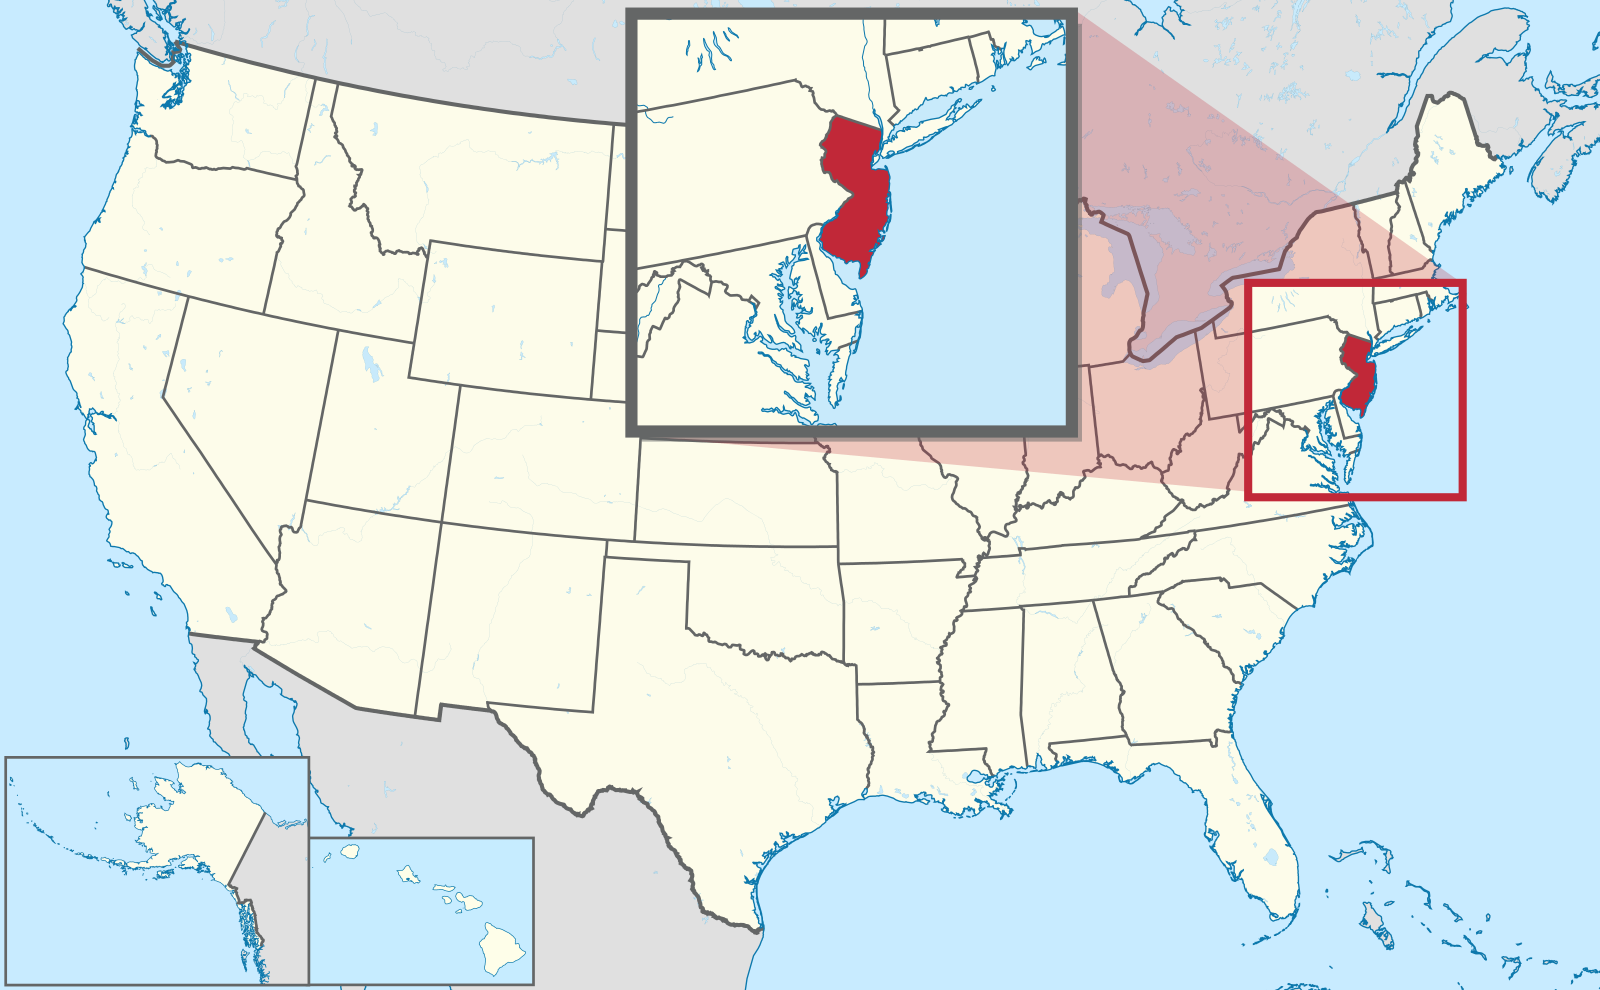
\includegraphics[width = \textwidth]{figures/nj_map}
\end{frame}

\begin{frame}
\begin{tikzpicture}[x = \textwidth, y = \textheight]
\node at (.5,.5) {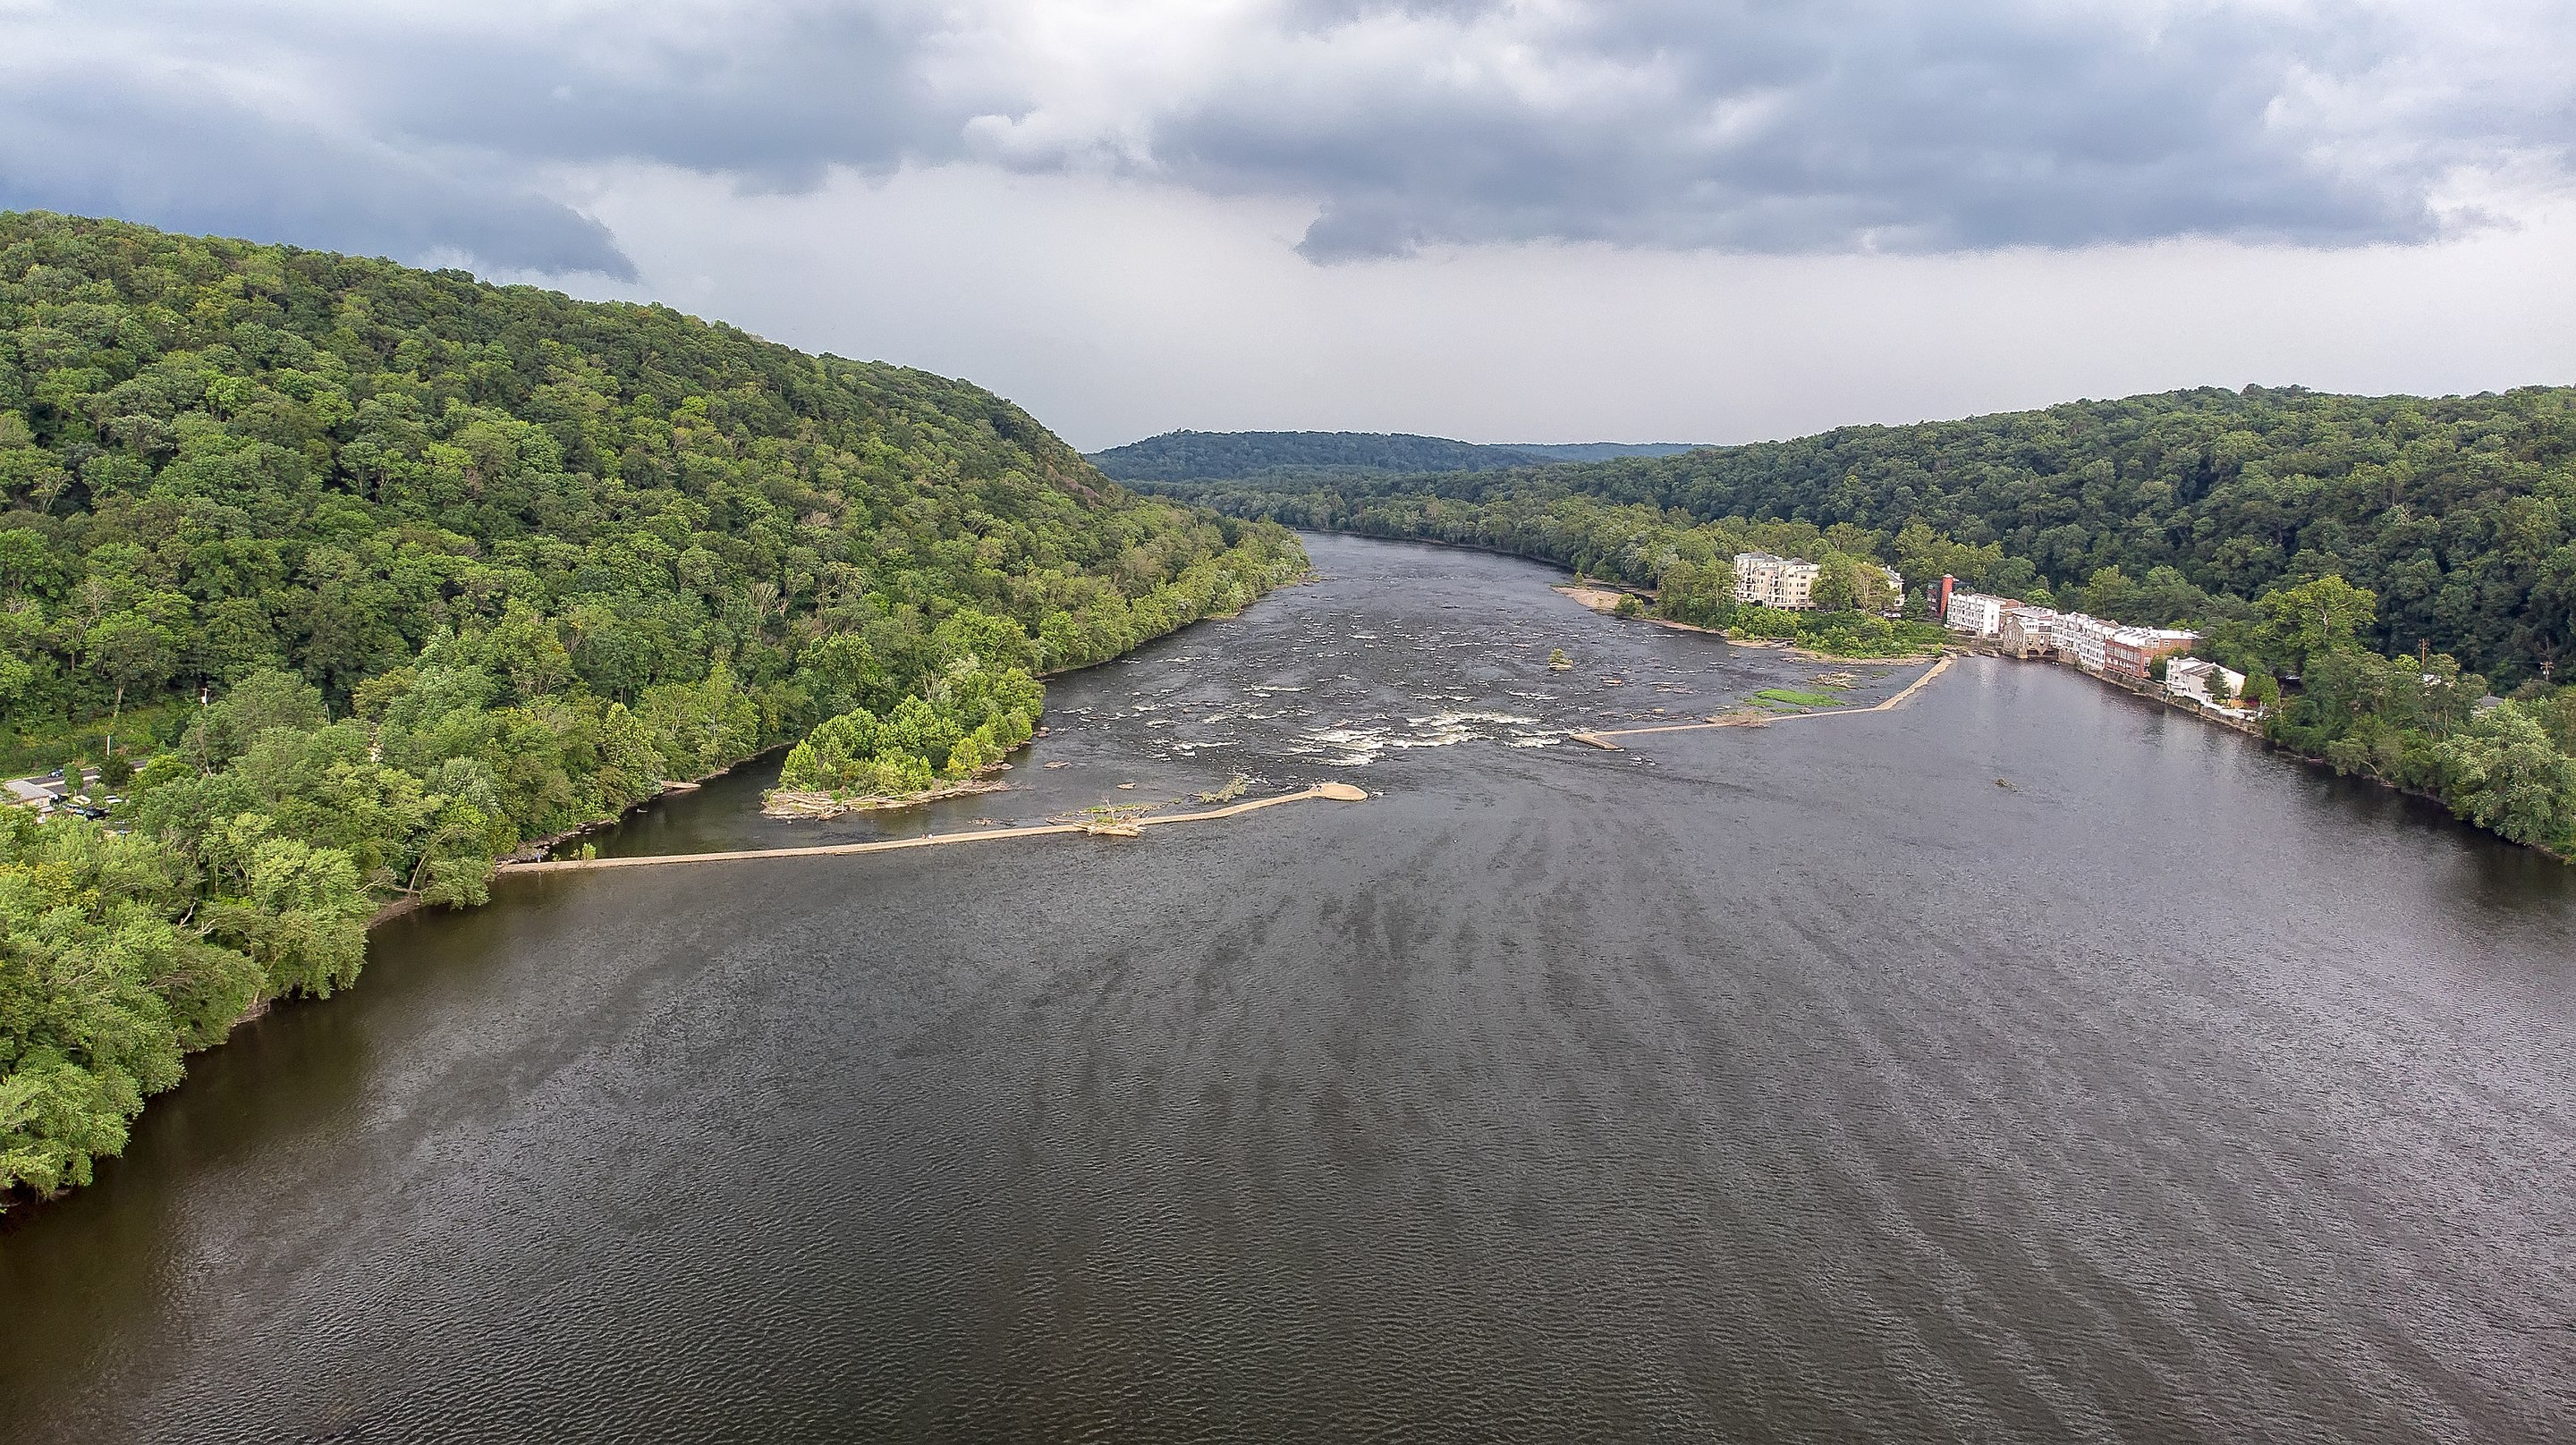
\includegraphics[width = \textwidth]{figures/Delaware_River}};
\node[anchor = south east, font = \tiny, align = center] at (1,0) {Photo by James Loesch - https://www.flickr.com/photos/jal33/49113053632/\\CC BY 2.0, https://commons.wikimedia.org/w/index.php?curid=87207834}; \pause
\node[anchor = north west, font = \bf, white, align = left] at (.03,.64) {New Jersey\\Minimum Wage\\Rose}; \pause
\node[anchor = north east, font = \bf, white, align = right] at (1,.64) {Pennsylvania\\No change};
\end{tikzpicture}
\end{frame}

\begin{frame}
\begin{tikzpicture}[x = \textwidth, y = \textheight]
\node at (0,0) {};
\node at (1,1) {};
\node[anchor = south] at (.2,.6) {
\includegraphics[width = .15\textwidth]{figures/burger_king}};
\node[anchor = south] at (.4,.6) {
\includegraphics[width = .15\textwidth]{figures/kfc}};
\node[anchor = south] at (.6,.6) {
\includegraphics[width = .15\textwidth]{figures/roy_rogers}};
\node[anchor = south] at (.8,.6) {
\includegraphics[width = .15\textwidth]{figures/wendys}};
\only<2->{
\node[anchor = north] at (.2,.6) {171 stores};
\node[anchor = north] at (.4,.6) {80 stores};
\node[anchor = north] at (.6,.6) {99 stores};
\node[anchor = north] at (.8,.6) {60 stores};
}
\only<3->{
\node[anchor = north west] at (0,.5) {Phone interview:};
\node[anchor = north west] at (.3,.5) {Feb-Mar 1992 before minimum wage rose};
\node[anchor = north west] at (.3,.44) {Nov-Dec 1992 after minimum wage rose};
}
\only<4->{
\node[anchor = north west] at (0, .35) {Recorded:};
\node[anchor = north west] at (.3, .35) {How many full-time equivalent employees?};
}
\end{tikzpicture}
\end{frame}

\begin{frame}
Did starting wages rise in NJ?
\end{frame}

\begin{frame}
\centering
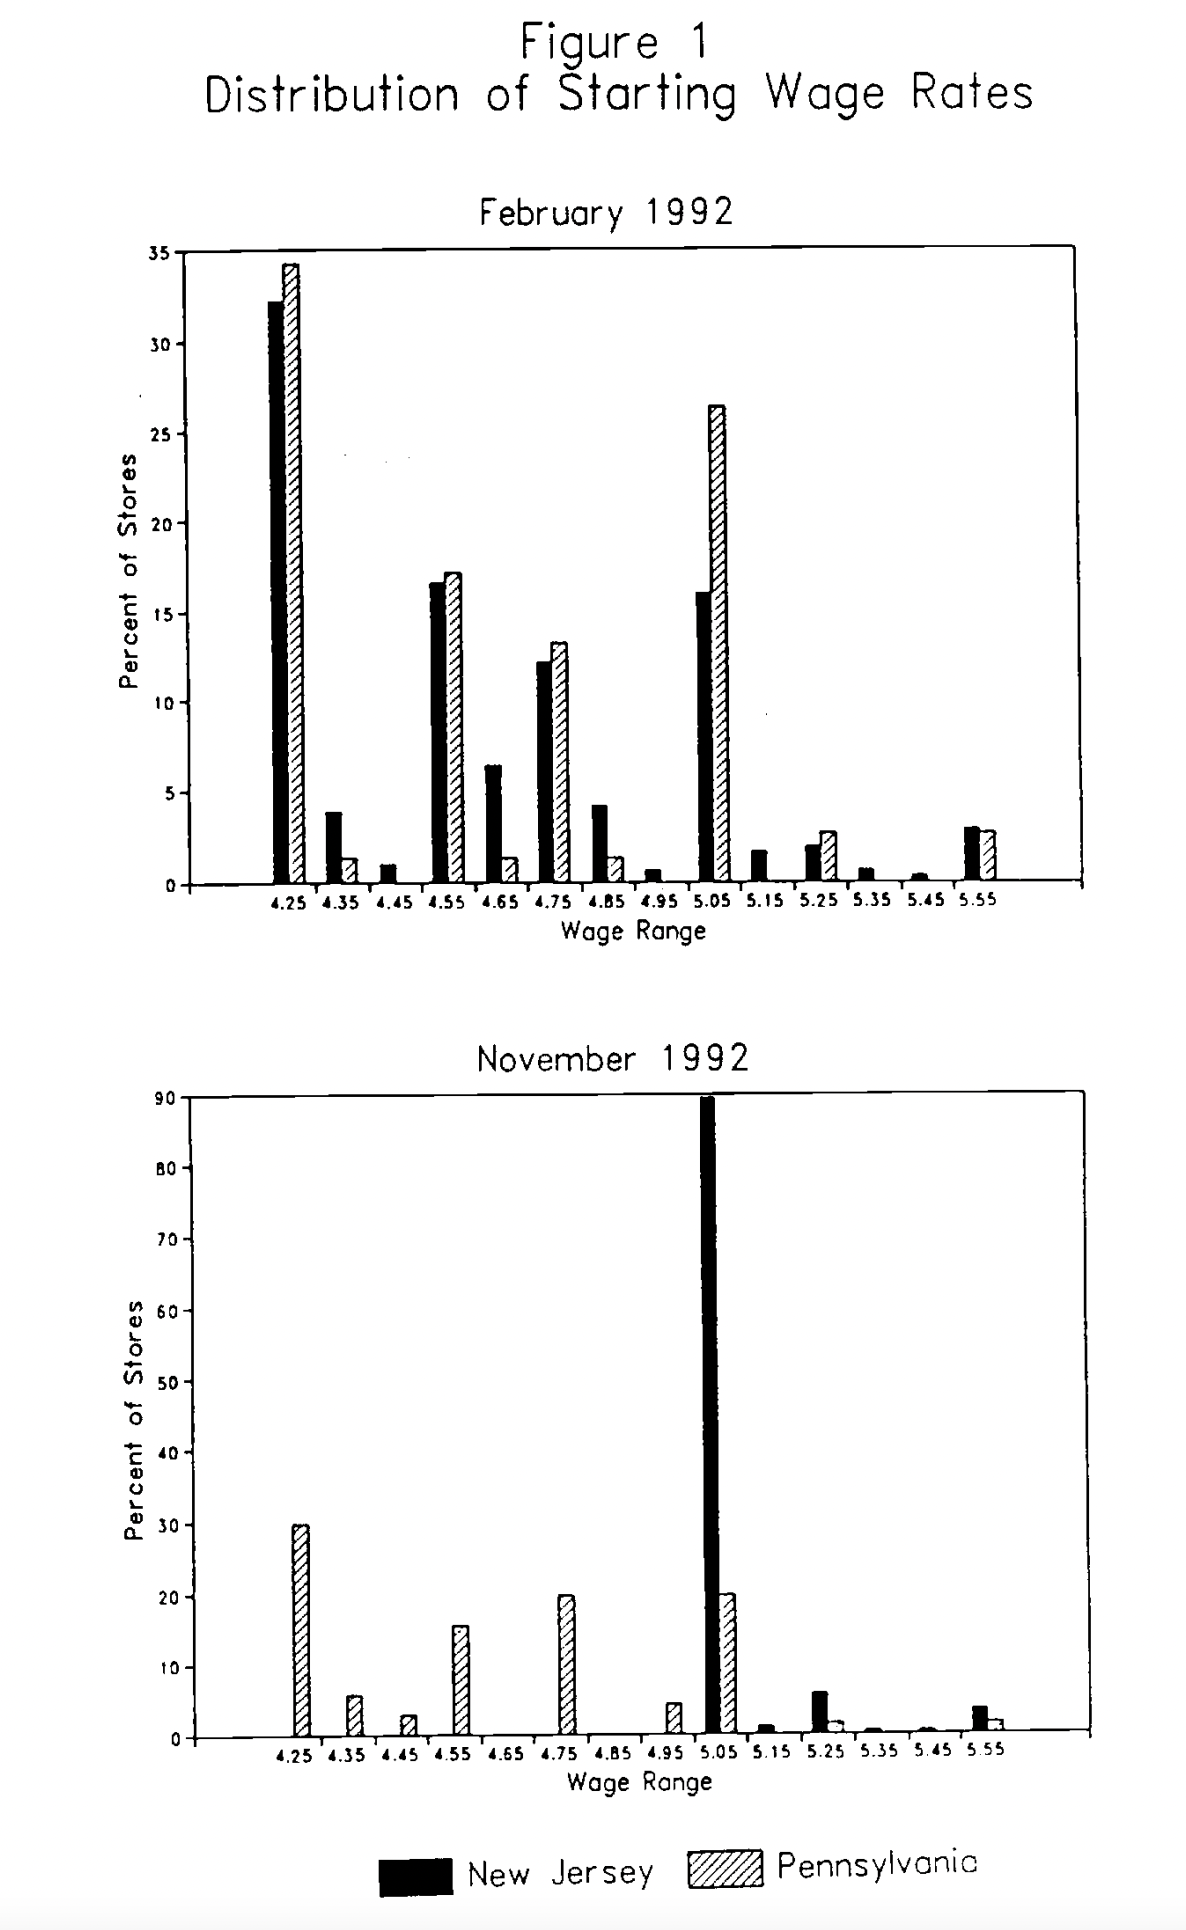
\includegraphics[height = \textheight]{figures/ck_fig1}
\end{frame}

\begin{frame}
How did employment change?
\end{frame}

\begin{frame}[t]

\includegraphics<1>[width = \textwidth]{figures/ck_slide1.pdf}
\includegraphics<2>[width = \textwidth]{figures/ck_slide2.pdf}
\includegraphics<3>[width = \textwidth]{figures/ck_slide3.pdf}
\includegraphics<4>[width = \textwidth]{figures/ck_slide4.pdf}
\includegraphics<5>[width = \textwidth]{figures/ck_slide5.pdf}

\end{frame}

\begin{frame}

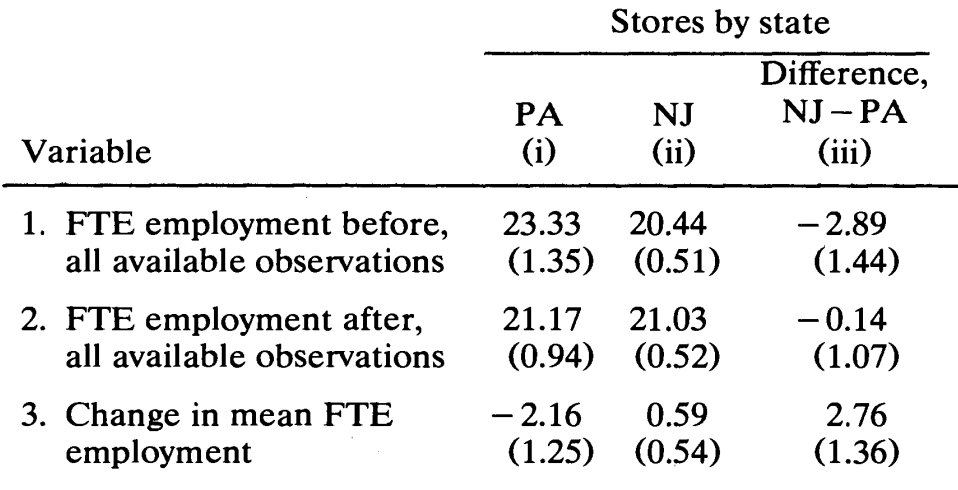
\includegraphics[width = .8\textwidth]{figures/ck_table}

\end{frame}

\begin{frame}

``Contrary to the central prediction of the textbook model of the minimum wage,...we find no evidence that the rise in New Jersey's minimum wage reduced employment at fast-food restaurants in the state.'' \vskip .5in

Card \& Krueger 1994, p.~792

\end{frame}

\begin{frame}

\begin{itemize}
\item simple study
\item well-executed
\item upended conventional wisdom
\end{itemize} \pause \vskip .2in
Decades of papers followed suit. Here is one.

\end{frame}

\begin{frame}

Malesky, E. J., Nguyen, C. V., \& Tran, A. (2014).\\
\bref{https://doi.org/10.1017/S0003055413000580}{The impact of recentralization on public services:\\A difference-in-differences analysis of the abolition of elected councils in Vietnam.}\\
American Political Science Review, 108(1), 144-168.

\end{frame}

\begin{frame}

Does government work better when it is centralized or decentralized?

\end{frame}

\begin{frame}{Vietnam setting: A study of recentralization}


\begin{tikzpicture}[x = \textwidth, y = .8\textheight]
\node at (0,0) {};
\node at (1,1) {};
\node[draw, rounded corners] (national) at (.45,.8) {National Assembly};
\node[draw, rounded corners] (provincial) at (.45,.6) {Provincial People's Committee};
\node[draw, rounded corners] (district) at (.45,.4) {District People's Committee};
\node[draw, rounded corners] (commune) at (.45,.2) {Commune People's Committee};
\draw[->, thick] (national) -- (provincial);
\draw[->, thick] (provincial) -- (district);
\draw[->, thick] (district) -- (commune);
\node[font = \footnotesize, anchor = east] at (1,.8) {most centralized};
\node[font = \footnotesize, anchor = east] at (1,.4) {district $\approx$ 120k people};
\node[font = \footnotesize, anchor = east] at (1,.2) {most decentralized};
\draw[line width = 2pt, red] (district.west) -- (district.east);
\node[font = \footnotesize, anchor = west, red, align = left] at (0,.4) {National Assembly\\2008 Resolution\\to Study\\Removal of DPCs};
\end{tikzpicture}

\end{frame}

\begin{frame}{Vietnam setting: A study of recentralization}

Input from social scientists \pause
\begin{enumerate}
\item Enough treated units to study \pause
\item Sampling stratified by region \pause
\item Sampling stratified by
\begin{itemize}
\item city versus rural
\item lowland versus highland
\item midland versus inter-nationally bordered land
\end{itemize} \pause
\item Sampling stratified by socioeconomic and public administration performance
\end{enumerate}

\end{frame}

\begin{frame}
\centering
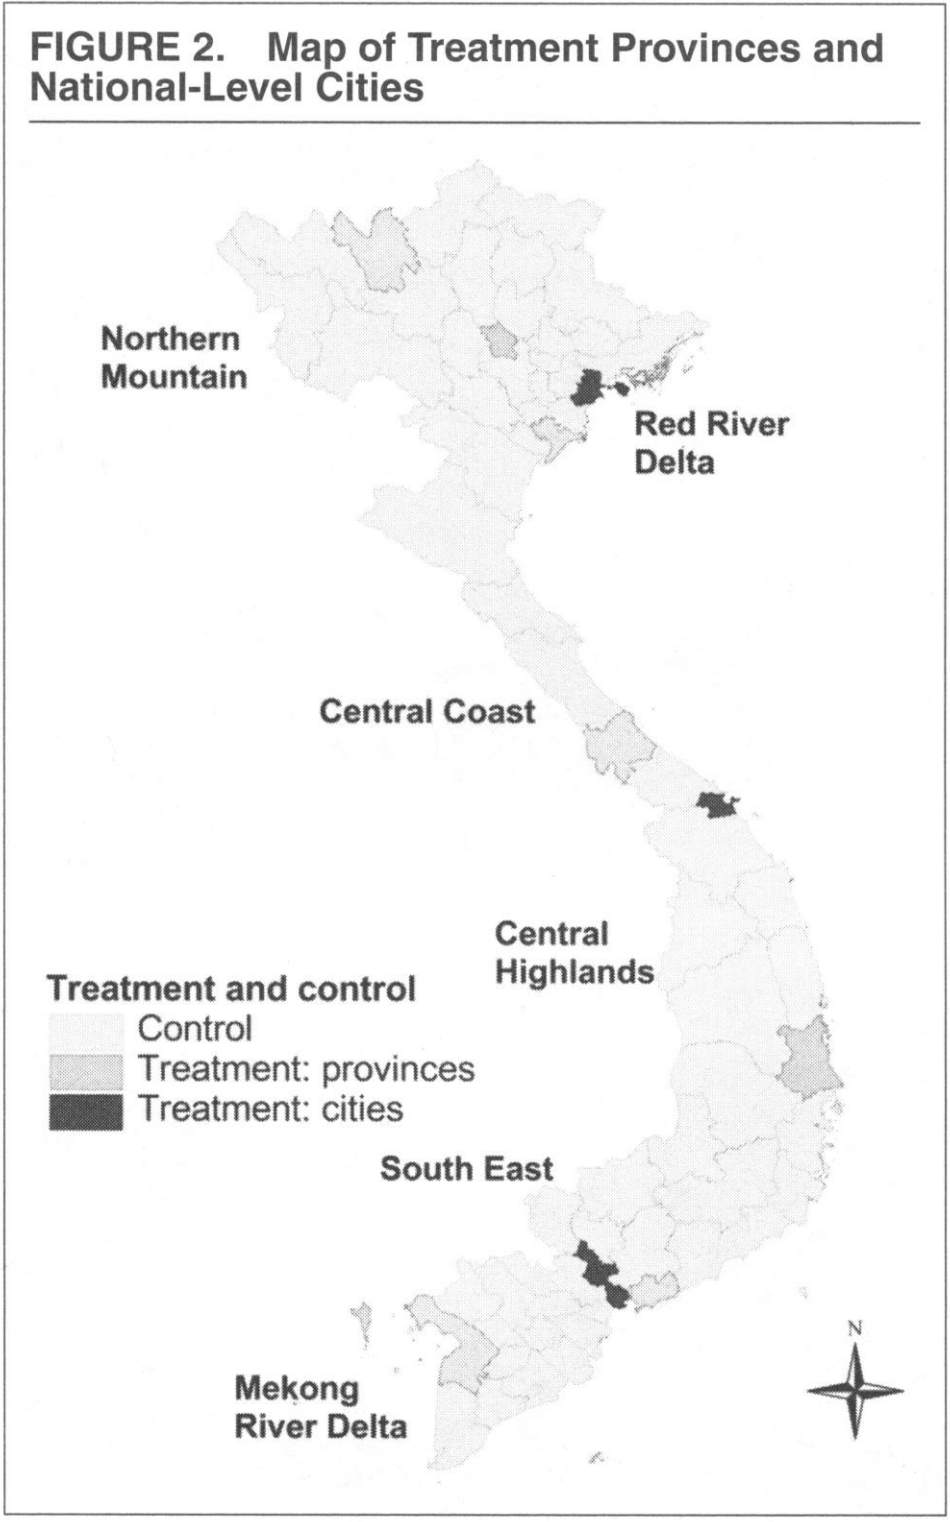
\includegraphics[height = .9\textheight]{figures/malesky_map}
\end{frame}

\begin{frame}

Vietnam Household Living Standards Survey\\
Reports by each local commune by commune leaders
\begin{itemize}
\item 2006 and 2008: Before DPC abolition
\item 2010: After DPC abolition
\end{itemize}
One outcome we will examine:\\
Is there the following project in the commune?
\begin{itemize}
\item Investment on culture and education
\end{itemize}

\end{frame}

\begin{frame}

\centering
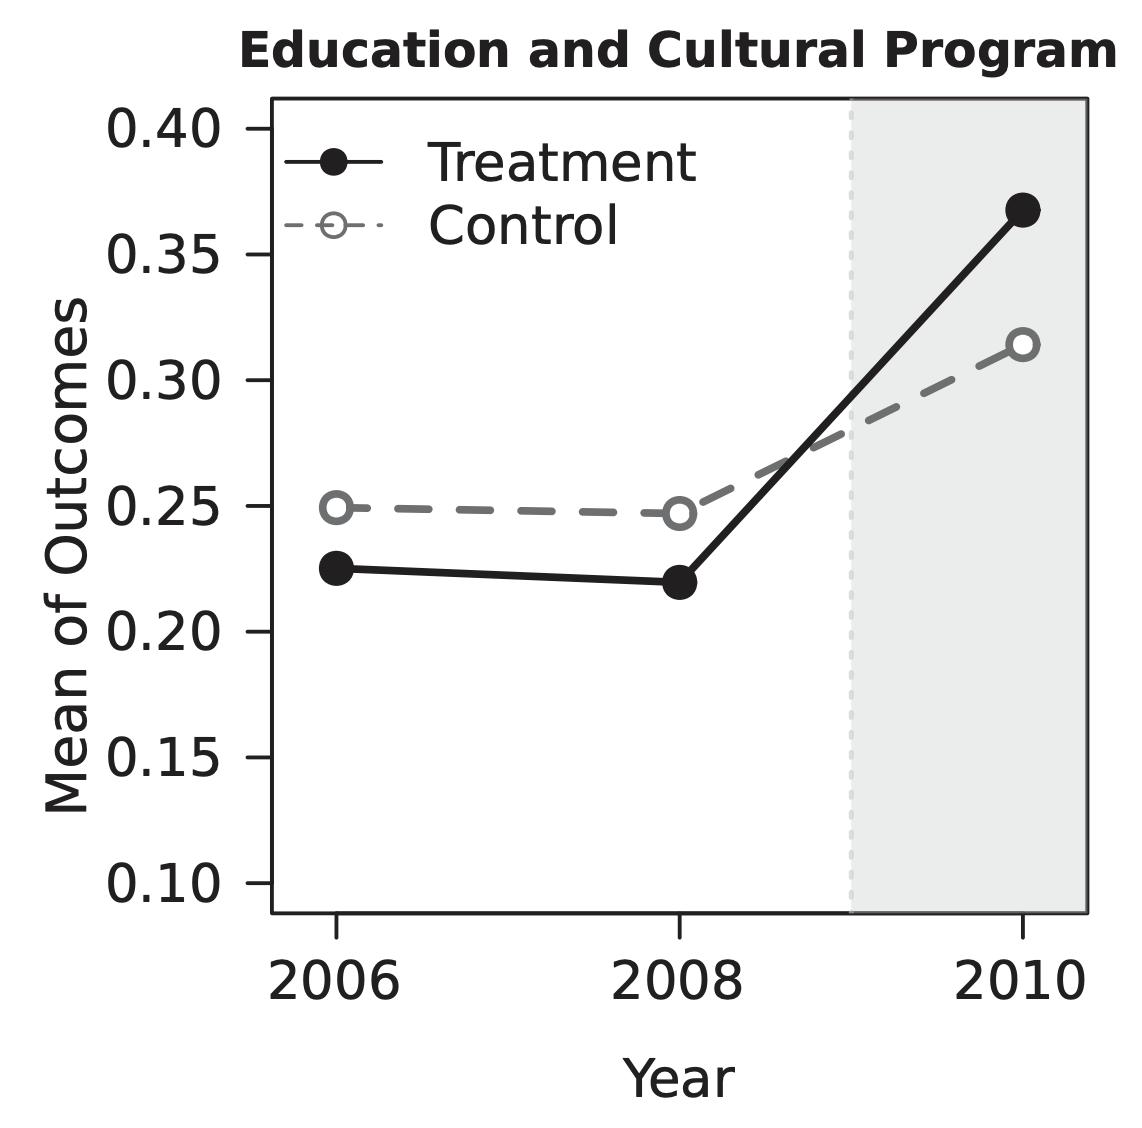
\includegraphics[width = .5\textwidth]{figures/egami_yamauchi_fig3a} \vskip .3in
\begin{footnotesize}
Screenshot of re-analysis by \bref{https://doi.org/10.1017/pan.2022.8}{Egami \& Yamauchi 2023}, Fig 3
\end{footnotesize}

\end{frame}

\begin{frame}{Difference in difference}

When no control unit is comparable to a treated unit,\\
we might assume a control unit and treated unit share\\
the same trend in the potential outcome under control

\begin{center}
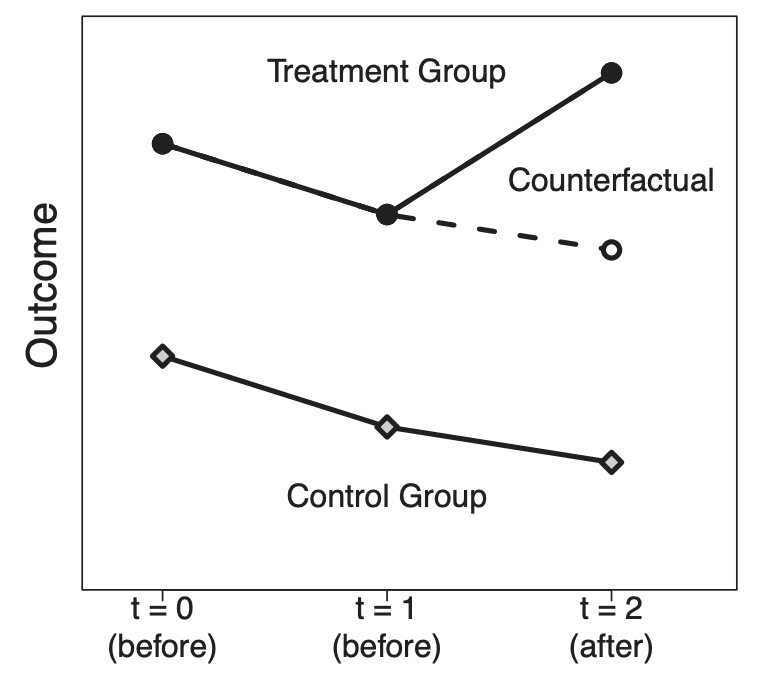
\includegraphics[width = .4\textwidth]{figures/egami_yamauchi_fig2a}
%\begin{tikzpicture}[x = 2in, y = 1.5in]
%\draw[<->, thick] (0,1) -- (0,0) -- (1,0);
%\draw[dashed] (.5,0) --  node[midway, right, align = left] {policy\\change} (.5,1);
%\end{tikzpicture}
\end{center}

\end{frame}

\goalsframe


\end{document}
